%%%%%%%%%%%%%%%%%%%%%%%%%%%%%%%%%%%%%%%%%
% a0poster Portrait Poster 
% LaTeX Template
% with University Copenhagen logo
% Version 1.0 (22/06/13)
%
% Based on:
% The a0poster class was created by:
% Gerlinde Kettl and Matthias Weiser (tex@kettl.de)
% 
% This template has been downloaded from:
% http://www.LaTeXTemplates.com
%
%%%%%%%%%%%%%%%%%%%%%%%%%%%%%%%%%%%%%%%%%

%----------------------------------------------------------------------------------------
%	PACKAGES AND OTHER DOCUMENT CONFIGURATIONS
%----------------------------------------------------------------------------------------

\documentclass[a0,portrait]{a0poster}
\usepackage[utf8]{inputenc}
\usepackage{multicol} % This is so we can have multiple columns of text side-by-side
\columnsep=100pt % This is the amount of white space between the columns in the poster
\columnseprule=3pt % This is the thickness of the black line between the columns in the poster

\usepackage[svgnames]{xcolor} % Specify colors by their 'svgnames', for a full list of all colors available see here: http://www.latextemplates.com/svgnames-colors

%\usepackage{times} % Use the times font
\usepackage{palatino} % Uncomment to use the Palatino font

\usepackage{url}
\usepackage{fancyvrb}
\usepackage{enumitem}

\usepackage{graphicx} % Required for including images
\graphicspath{{figures/}} % Location of the graphics files
\usepackage{booktabs} % Top and bottom rules for table
\usepackage[font=small,labelfont=bf]{caption} % Required for specifying captions to tables and figures
\usepackage{amsfonts, amsmath, amsthm, amssymb} % For math fonts, symbols and environments
\usepackage{wrapfig} % Allows wrapping text around tables and figures
\definecolor{ku}{RGB}{144,26,30}
\definecolor{ku-yellow}{RGB}{255,249,25}
\definecolor{grey}{RGB}{100, 100, 100}
\definecolor{darkgreen}{RGB}{0, 0.2, 0.13}

 \usepackage{eso-pic}
               \newcommand\BackgroundIm{
               \put(66,-41){
               \parbox[b][\paperheight]{\paperwidth}{%
               \vfill
               \centering
               \includegraphics[height=\paperheight,width=\paperwidth,
               keepaspectratio]{background.pdf}%
               \vfill
               }}}

\usepackage[top=2in, bottom=0in, left=2in, right=0.2in]{geometry}
\usepackage{titlesec}
\titlespacing*{\section}{0cm}{1cm}{0.5cm}
\setlength{\parindent}{1cm}

\begin{document}
 \AddToShipoutPicture*{\BackgroundIm}
%----------------------------------------------------------------------------------------
%	POSTER HEADER 
%----------------------------------------------------------------------------------------

% The header is divided into two boxes:
% The first is 75% wide and houses the title, subtitle, names, university/organization and contact information
% The second is 25% wide and houses a logo for your university/organization or a photo of you
% The widths of these boxes can be easily edited to accommodate your content as you see fit

\begin{minipage}[t]{0.78\linewidth}
\vspace{10cm}
\Huge \color{ku} \textbf{Volr: A declarative interface language for neural computation} \color{Black}\\[-1.8cm] % Title
\huge\textit{Experimental neural systems modeling with Jupyter Notebooks}\\[1cm] % Subtitle
\begin{tabular}{l@{\hspace{1in}}l}
\Large \textbf{Jens Egholm Pedersen} & \Large \textbf{Christian Pehle}\\ % Author(s)
\Large Department of Computer Science & \Large Kirchoff-Institute for Physics\\ % University/organization
\Large University of Copenhagen & \Large University of Heidelberg
\end{tabular}

\end{minipage}
%
\begin{minipage}[t]{0.22\linewidth}
\vspace{13.5cm}
\flushright
\color{DarkSlateGray}
\Large \textbf{Contact Information:}\\
Universitetsparken 5 \\
2100 København Ø\\[1cm]
+45 25122752\\ % Phone number
\texttt{xtp778@alumni.ku.dk}% Email address
\end{minipage}

\vspace{0.5cm} % A bit of extra whitespace between the header and poster content

%----------------------------------------------------------------------------------------

\begin{multicols}{2} % This is how many columns your poster will be broken into, a portrait poster is generally split into 2 columns

%----------------------------------------------------------------------------------------
%	ABSTRACT
%----------------------------------------------------------------------------------------

\color{ku} % Navy color for the abstract

\begin{abstract}

\noindent For researchers with little to no programming experience, NEST can be intimidating. Despite the efforts done by the NEST community to adopt interface libraries like PyNN, pre-and post-processing remains time-consuming and complicated. By drawing on concise abstractions and tools such as connection-set algebra and Jupyter notebooks, a holistic execution environment has the potential to lower the barrier to entry and drastically increase the adoption of NEST. Developed in collaboration with cognitive neuroscientists, a domain-specific language and a Jupyter notebook plugin is presented. It establishes a single execution environment, to act as an intermediate layer between the researcher and the simulation. The environment builds on the efforts of PyNN and has been demonstrated to work with both NEST and BrainScaleS. Future plans are to integrate high level abstractions for learning in the domain-specific language, making use of the learning-to-learn paradigm.
\end{abstract}

%----------------------------------------------------------------------------------------
%	INTRODUCTION
%----------------------------------------------------------------------------------------
\color{SaddleBrown} % SaddleBrown color for the introduction
\section*{Introduction}
Despite the pioneering work of simulator APIs for neural experiments, there are still 
significant barriers to entry for inexperienced users: learning an interface language like 
PyNN (including comprehending the theoretical counterparts), digitising analog experiments and 
performing complicated pre- and post-processing of large amounts of data.

The showcased project presents a prototype of a development environment for experimenting 
with neural simulations.
The domain-specific language (DSL) Volr offers a concise method for specifying experiments,
while the execution environment around Volr integrates seamlessly with Jupyter Notebooks and 
several execution targets like NEST. 
The project makes working with neural simulations simpler and more efficient, thereby
increasing the research output and widening the audience for neural simulators. 

The prototype is designed to facilitate the entire life cycle of an experiment: 
generation/preprocessing of data, neural network topology and properties, experimental setup 
and finally data extraction and post-processing (see figure \ref{fig:model}).\\[0.4cm]
\indent Documentation is available at: \hspace{0.5cm} \textbf{\texttt{https://volr.readthedocs.io}}

% 
%----------------------------------------------------------------------------------------
%	OBJECTIVES
%----------------------------------------------------------------------------------------

\color{DarkSlateGray} % DarkSlateGray color for the rest of the content

\section*{Project objectives}

\begin{enumerate}[itemsep=1mm]
\item Integrate with evaluation platforms for simulated, neuromorphic and artificial neural networks.
\item Support fast feedback loops between experimental ideas and results.
\item Develop a concise and formal declarative language to reproduce and reason about experiments.
\item Explore the domain space for cognitive experiments including learning and online plasticity.
\end{enumerate}

\begin{center}\vspace{0.3cm}
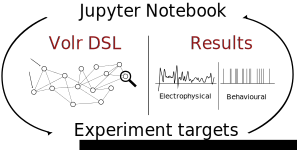
\includegraphics[width=0.9\linewidth]{volr_model}
\captionof{figure}{The workflow of an entire experiment, from the modeling in a 
				   Jupyter notebook, through the evaluation on one or more platforms,
                   to the retrieving of the experiment results  
                   for subsequent analysis. From the perspective of the user
                   everything happens directly in the notebook.}
\label{fig:model}
\end{center}

\section*{1. Execution targets}
The current prototype integrates with three simulation targets: NEST (through the NEST API), 
BrainScaleS for spiking neural networks (SNN) (through PyNN) and artificial neural networks 
(ANN) with GPU acceleration (through Futhark \cite{Henriksen2017}).

The DSL maintains an intermediate representation of the experiments, including all the 
necessary details to reproduce the setup.
Generated specifications exist for all execution targets to correctly map the experiment
to running code.
This lets Volr expose constraints directly in the language to provide conveniences like
compile-time model verification.

Finally, the intermediate representation simplifies the integration with execution targets,
currently by through the efforts of Futhark, PyNN and the NEST API (see figure
\ref{fig:pipeline}).
However other targets would be interesting to examine, such as SpiNNaker, TensorFlow, Intel's 
Loihi chip and the next generation BrainScaleS 2 system from Heidelberg.

\begin{center}\vspace{1.3cm}
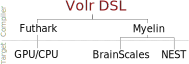
\includegraphics[width=0.9\linewidth]{volr_pipeline}
\captionof{figure}{The translation from the DSL to the execution targets. ANN models are
                   interpreted by Futhark which in turn is evaluated on GPU/CPUs.
                   SNN models are interpreted by the internal Myelin compiler that checks
                   for inconsistencies and generates target-specific code through PyNN and
                   the NEST API.}
\label{fig:pipeline}
\end{center}

\section*{2. Fast experiment feedback loop with Jupyter Notebooks}
Jupyter Notebooks are increasingly popular in data processing and data analysis domains.
The interactive and iterative approach allows researchers to quickly map hypotheses 
to experiments, with the support of the vast Python ecosystem.

After installing the environment it takes less than a minute to setup an experiment and
extract the first results. 
Figure \ref{fig:experiment} illustrates how data can be injected and extracted.
By building on open technologies like Python and Jupyter Notebooks, the experiments are
straight-forward to share and expand upon.

\begin{center}
\vspace{-0.3cm}
\begin{multicols}{2}
\renewcommand{\theFancyVerbLine}{\small \arabic{FancyVerbLine}}
\centering
a) Generating experiment input
\begin{Verbatim}[numbers=left,xleftmargin=5mm,commandchars=\\\{\}]
\textbf{\color{ku}in_stim} = ... \color{grey}# Spikes or data 

\textbf{\color{ku}stimulus}\color{black} s
  input: \textbf{$in_stim}
\end{Verbatim}

b) Analysing experiment output
\begin{Verbatim}[numbers=left,xleftmargin=5mm,commandchars=\\\{\}]
\color{grey}# Plot experiment data\color{black}
\textbf{result}.spikes.plot()
\color{grey}# Plot target specific data\color{black}
\textbf{result}.nest.voltages.plot()
\end{Verbatim}
\end{multicols}
\vspace{-0.4cm}
\captionof{figure}{Examples for a) injecting experimental data 
                   and b) extracting plots with Python.}
\label{fig:experiment}
\end{center}

\section*{3. DSL specification and design}
\setlength{\columnsep}{2cm}
\begin{wrapfigure}{r}{11cm}
\vspace{-0.9cm}
\renewcommand{\theFancyVerbLine}{\small \arabic{FancyVerbLine}}
\begin{Verbatim}[numbers=left,xleftmargin=5mm,commandchars=\\\(\)]
\textbf(\color(ku)stimulus)\color(black) s
  input: "data.json"
\textbf(\color(ku)population) p
  from s: one to one
  neurons: 20
\textbf(\color(ku)response)\color(black)
  from p: all to one
\textbf(\color(ku)target)\color(black) NEST
  model: izhikevich
\textbf(\color(ku)target)\color(black) BrainScaleS
  model: if_cond_exp
\end{Verbatim}
\vspace{-0.4cm}
\captionof{figure}{A simple experimental setup using the Izhikevich neuron model
                   on NEST and an integrate-and-fire model on BrainScales.}
\label{fig:volr}
\vspace{-3cm}
\end{wrapfigure}

\noindent At the core of project is the domain-specific language (DSL) Volr, that models neural network 
topology as well as simulator-specific properties. 
The DSL is built in Haskell and seeks to form the basis for a tailor-made modeling language 
for the cognitive and theoretical neuroscience \cite{Innes2017}.

The inner representational structure allows for abstract analyses, by understanding networks
as first-class citizens subject to function composition and lambda calculus.
These \textit{algebraic} properties could pave the way for the application of techniques
such as reverse differentiation, dependent types and semantic error checking.

The syntax of the DSL is showcased in figure \ref{fig:volr}.
It supports detailed descriptions of population and neuron properties and employs
connection-set algebra to model connectivity \cite{Djurfeldt2012}.

\section*{4. Future work}
In collaboration with the Unit for Cognitive Neuroscience at Copenhagen University the 
current prototype is employed to study computational models of cognitive rehabilitation 
theories.
Volr gives cognitive neuroscientists a larger degree of independence, while letting them
construct complex experiments without the need for intimate knowledge of the execution 
targets.

Learning-to-learn is a technique for training a SNN with a similar ANN using gradient
analysis. Because of the easy translation between artificial and spiking models in Volr, the
learning-to-learn framework would be ideal to explore further \cite{Bellec2018}.

Lastly the algebraic properties of the internal model deserve to be explored. Techniques
such as automatic differentiation could permit the fast generation of large and complex
SNN \cite{Baydin2018}.

%----------------------------------------------------------------------------------------
%	CONCLUSIONS
%----------------------------------------------------------------------------------------

\color{SaddleBrown} % SaddleBrown color for the conclusions to make them stand out

\section*{Conclusions}

\begin{enumerate}
\item Prototypical integration with Jupyter Notebooks has been shown to allow fast iterations of experiments, with immediate access to already familiar Python tools for large-scale data analysis.
\item The formalised domain-specific language, Volr, has been developed to describe reproducible and consistent neural network experiments for artificial and spiking substrates.
It exploits algebraic techniques such as connection-set algebra \cite{Djurfeldt2012} and network-function compositions.
\item Three targets are currently supported: NEST, BrainScales and artificial neural networks through Futhark. Further work is needed to expand existing targets and include platforms such as Intel's Loihi, SpiNNaker and the new DLS chip from Heidelberg, Germany.
\item Ongoing work is exploring the domain of more complex cognitive experiments, including 
the possibility for \textit{learning-to-learn} integration between ANN and SNN, cognitive 
tasks modeling and reverse differentiation for ANN.
\end{enumerate}

\color{DarkSlateGray} % Set the color back to DarkSlateGray for the rest of the content

 %----------------------------------------------------------------------------------------
%	REFERENCES
%----------------------------------------------------------------------------------------

\nocite{*} % Print all references regardless of whether they were cited in the poster or not
\bibliographystyle{plain} % Plain referencing style
\bibliography{sample} % Use the example bibliography file sample.bib

%----------------------------------------------------------------------------------------
%	ACKNOWLEDGEMENTS
%----------------------------------------------------------------------------------------

\section*{Acknowledgements}
We are grateful for the valuable time and counsel of Sebastian Schmitt and Karlheinz Meier 
from the Kirchoff-Institute for Physics at the University of Heidelberg, Germany.

We would like to thank Jesper Mogensen and Nicolai Daugaard from the Unit for Cognitive 
Neuroscience and Martin Elsman from the Department of Computer Science at the University of 
Copenhagen for their interest and important contributions to the project.

%----------------------------------------------------------------------------------------

\end{multicols}
\end{document}


%\subsection*{Mathematical Section}
%Nulla vel nisl sed mauris auctor mollis non sed. 

%\begin{equation}
%E = mc^{2}
%\label{eqn:Einstein}
%\end{equation}

% Curabitur mi sem, pulvinar quis aliquam rutrum. (1) edf (2)
% , $\Omega=[-1,1]^3$, maecenas leo est, ornare at. $z=-1$ edf $z=1$ sed interdum felis dapinbus sem. $x$ set $y$ ytruem. 
% Turpis $j$ amet accumsan enim $y$-lacina; 
% ref $k$-viverra nec porttitor $x$-lacina. 

% Vestibulum ac diam a odio tempus congue. Vivamus id enim nisi:

% \begin{eqnarray}
% \cos\bar{\phi}_k Q_{j,k+1,t} + Q_{j,k+1,x}+\frac{\sin^2\bar{\phi}_k}{T\cos\bar{\phi}_k} Q_{j,k+1} &=&\nonumber\\ 
% -\cos\phi_k Q_{j,k,t} + Q_{j,k,x}-\frac{\sin^2\phi_k}{T\cos\phi_k} Q_{j,k}\label{edgek}
% \end{eqnarray}
% and
% \begin{eqnarray}
% \cos\bar{\phi}_j Q_{j+1,k,t} + Q_{j+1,k,y}+\frac{\sin^2\bar{\phi}_j}{T\cos\bar{\phi}_j} Q_{j+1,k}&=&\nonumber \\
% -\cos\phi_j Q_{j,k,t} + Q_{j,k,y}-\frac{\sin^2\phi_j}{T\cos\phi_j} Q_{j,k}.\label{edgej}
% \end{eqnarray} 

% Nulla sed arcu arcu. Duis et ante gravida orci venenatis tincidunt. Fusce vitae lacinia metus. Pellentesque habitant morbi. $\mathbf{A}\underline{\xi}=\underline{\beta}$ Vim $\underline{\xi}$ enum nidi $3(P+2)^{2}$ lacina. Id feugain $\mathbf{A}$ nun quis; magno.

% %----------------------------------------------------------------------------------------
% %	RESULTS 
% %----------------------------------------------------------------------------------------

% \section*{Results}

% Donec faucibus purus at tortor egestas eu fermentum dolor facilisis. Maecenas tempor dui eu neque fringilla rutrum. Mauris \emph{lobortis} nisl accumsan. Aenean vitae risus ante.
% %
% \begin{wraptable}{l}{12cm} % Left or right alignment is specified in the first bracket, the width of the table is in the second
% \begin{tabular}{l l l}
% \toprule
% \textbf{Treatments} & \textbf{Response 1} & \textbf{Response 2}\\
% \midrule
% Treatment 1 & 0.0003262 & 0.562 \\
% Treatment 2 & 0.0015671 & 0.910 \\
% Treatment 3 & 0.0009271 & 0.296 \\
% \bottomrule
% \end{tabular}
% \captionof{table}{\color{Green} Table caption}
% \end{wraptable}
% %
% Phasellus imperdiet, tortor vitae congue bibendum, felis enim sagittis lorem, et volutpat ante orci sagittis mi. Morbi rutrum laoreet semper. Morbi accumsan enim nec tortor consectetur non commodo nisi sollicitudin. Proin sollicitudin. Pellentesque eget orci eros. Fusce ultricies, tellus et pellentesque fringilla, ante massa luctus libero, quis tristique purus urna nec nibh.

% Nulla ut porttitor enim. Suspendisse venenatis dui eget eros gravida tempor. Mauris feugiat elit et augue placerat ultrices. Morbi accumsan enim nec tortor consectetur non commodo. Pellentesque condimentum dui. Etiam sagittis purus non tellus tempor volutpat. Donec et dui non massa tristique adipiscing. Quisque vestibulum eros eu. Phasellus imperdiet, tortor vitae congue bibendum, felis enim sagittis lorem, et 

% In hac habitasse platea dictumst. Etiam placerat, risus ac.

% Adipiscing lectus in magna blandit:

% \begin{center}\vspace{1cm}
% \begin{tabular}{l l l l}
% \toprule
% \textbf{Treatments} & \textbf{Response 1} & \textbf{Response 2} \\
% \midrule
% Treatment 1 & 0.0003262 & 0.562 \\
% Treatment 2 & 0.0015681 & 0.910 \\
% Treatment 3 & 0.0009271 & 0.296 \\
% \bottomrule
% \end{tabular}
% \captionof{table}{\color{Green} Table caption}
% \end{center}\vspace{1cm}

% Vivamus sed nibh ac metus tristique tristique a vitae ante. Sed lobortis mi ut arcu fringilla et adipiscing ligula rutrum. Aenean turpis velit, placerat eget tincidunt nec, ornare in nisl. In placerat.
